\documentclass{standalone}
\usepackage{tikz}
\usetikzlibrary{mindmap}

\begin{document}

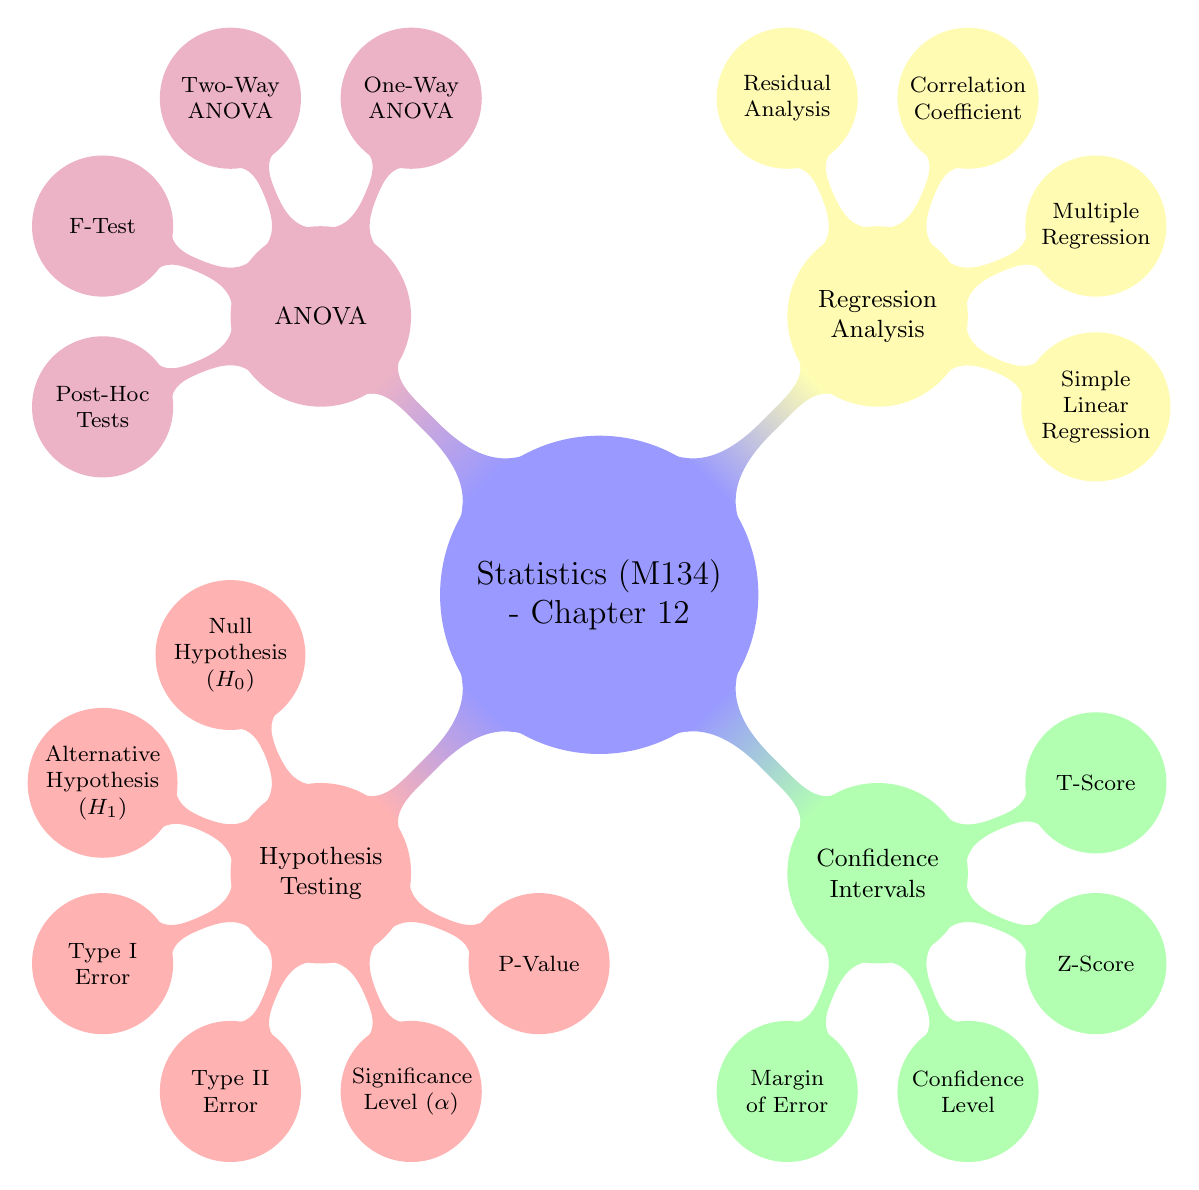
\begin{tikzpicture}[mindmap, grow cyclic, every node/.style=concept, concept color=blue!40, 
    level 1/.append style={level distance=5cm,sibling angle=90},
    level 2/.append style={level distance=3cm,sibling angle=45}]
    
    \node{Statistics (M134) - Chapter 12}
        child [concept color=red!30] { node {Hypothesis Testing}
            child { node {Null Hypothesis ($H_0$)} }
            child { node {Alternative Hypothesis ($H_1$)} }
            child { node {Type I Error} }
            child { node {Type II Error} }
            child { node {Significance Level ($\alpha$)} }
            child { node {P-Value} }
        }
        child [concept color=green!30] { node {Confidence Intervals}
            child { node {Margin of Error} }
            child { node {Confidence Level} }
            child { node {Z-Score} }
            child { node {T-Score} }
        }
        child [concept color=yellow!30] { node {Regression Analysis}
            child { node {Simple Linear Regression} }
            child { node {Multiple Regression} }
            child { node {Correlation Coefficient} }
            child { node {Residual Analysis} }
        }
        child [concept color=purple!30] { node {ANOVA}
            child { node {One-Way ANOVA} }
            child { node {Two-Way ANOVA} }
            child { node {F-Test} }
            child { node {Post-Hoc Tests} }
        };
\end{tikzpicture}

\end{document}